\documentclass[a4paper,10pt]{article}
\usepackage[utf8]{inputenc}
\usepackage{fullpage}
\usepackage{color}
\usepackage{authblk}
\usepackage{listings}
\usepackage{graphicx}
\usepackage{subcaption}
\usepackage{amsmath}
%PREPRINT/MANUSCRIPT OPTIONS
\usepackage{setspace}
\usepackage{lineno}
\linenumbers
\doublespacing

%opening

% \author{
%     \IEEEauthorblockN{James Gilbert\IEEEauthorrefmark{1}, Nicole Pearcy\IEEEauthorrefmark{1}, Jamie Twycross\IEEEauthorrefmark{2}}
%     \IEEEauthorblockA{\IEEEauthorrefmark{1}Synthetic Biology Research Centre, School of Life Sciences, University of Nottingham}
%     \IEEEauthorblockA{\IEEEauthorrefmark{2}Intelligent Modelling and Analysis Group, School of Computer Science, University of Nottingham}
% }

\begin{document}

\title{From clusters to queries: exploiting uncertainty in the modular landscape of complex networks}

%\titlerunning{Short form of title}        % if too long for running head

\author{James P Gilbert         \and
	Jamie Twycross 		\and
	John King
	}
\date{Received: date / Accepted: date}


\maketitle

\begin{abstract}
Uncovering latent community structure in complex networks is a field that has received an enormous amount of attention.
Unfortunately, whilst potentially very powerful unsupervised methods for classifying nodes into similar groups based on topology alone has been shown to have several major limitations.
Crucially, the search space for module extraction approaches appears to be extremely glassy, with many high valued solutions that lack any real similarity to one another.
However, in this paper we argue that this is not a flaw with the modularity maximisation algorithm but, rather, information that can be used to aid the classification of functional relationships between vertices.
Formally, we present an approach to generating a search ``index'' for a network, based on the space of high value modular partitions.
This search spaces allows the formulation of query based measures that provide a score for the level of relatedness to a given labelled query set.
The methods developed in this paper are applied to biological and social datasets with ground-truth label data, with very small query sets for nodes.
When tested on both real and synthetic datasets our method achieves extremely high levels of classification.
Furthermore, the approach can be applied in distributed environments potentially allowing it to scale to very large networks.
\end{abstract}

\section{Introduction}

A fundamental issue at the heart of machine learning methods applied to large scale datasets is the ability to correctly identify classes of related objects in an unsupervised manner.
In network science, this methodology is often referred to as \textit{community} detection, due to the intuitive analogy from the social sciences \cite{fortunato2010community}.
Many algorithms exist to solve this problem, yet initial starting conditions or different optimisation strategies may result in conflicting results even when the same objective function is being maximised \cite{good2010performance}.
In this paper, we develop an intuitive method to use the uncertainty amongst a high number of near optimal solutions to measure the overall quality of a given labelling scheme that can come from classes known \textit{a-priori} or clusters detected through other methods.
This approach also allows the expansion of labels to find potentially related vertices to an initial starting subset.

The number and size of communities is, generally, not known \textit{a priori}, and the problem has been shown to be NP-hard.
The work of Good \textit{et al.} \cite{good2010performance} recently highlighted that the popular modularity maximisation algorithm has a highly ``glassy'' search space.
In this situation there are many locally optimal partitions that bear little to no resemblance to each other by measure of mutual information.
This allows greedy optimisation algorithms \cite{blondel2008fast} to trivially find solutions that score extremely high values of modularity.
In order to solve this issue, certain approaches use a consensus based approach to clustering, combining many high value partitions into a given median partition.

Though the methods presented here can be applied to any complex network, the focus of this work is biological in nature; characterising the function of all genes within an organism is a problem critical to systems biology \cite{}.
In many situations, only the role of a small number of genes is known, with much of the annotation for a given organism being computed through naive homology information that ignores the role of a gene within a wider context.
The advent of high throughput experimental datasets has allowed the construction of genome scale networks, leading to the observation of non-trivial topological properties such as densely connected clusters \cite{ArabidopsisConsortium2011}.
These densely connected clusters are widely believed to be associated with specific function, such as protein complexes or biochemical pathways \cite{}.

This, and work in related fields, has led to the desire for computational techniques that elucidate related, modular structure in the form of community detection algorithms \cite{fortunato2010community}.
As a form of unsupervised machine learning module extraction methods largely focus on optimising some objective function with the desire of finding meaningful clusterings.
Perhaps the most popular of these methods is that of modularity maximisation \cite{newman2004}, which seeks to find the most unexpected partition of a graph with respect to a given null model.
One limitation of partition based methods is that each vertex can only belong to a community.
Overlapping methods have recently been applied to this problem in both \textit{crisp} \cite{ahn2010link, lancichinetti2011finding} and \textit{fuzzy} \cite{gregory2011fuzzy} based algorithms.


In this paper, we do not seek to find a single ``best'' partition, either overlapping or not.
Instead, we use the large number of highly modular solutions to form the index for a search query system.
In essence, this is a method of semi-supervised learning that attempts to find items related given labelled sets of vertices using topology alone.
Each high value partition, if statistically more modular than random, can be treated as information about the relationships between vertices.
As the objective of community detection approaches is to relate information, it is assumed that some labelled meta-data can be used to find unlabelled, potentially related vertices.
The overall objective can be thought of as a form of recommender system \cite{ricci2011introduction}, relating a given query in the form of a vertex set to potentially related information by exploiting the co-occurrence between communities.

In this vein, we apply the method presented in this paper to the problem of classifying biological function.
The objective of our algorithm, in this sense, is given sets of known function for genes or proteins within interaction networks, to generate meaningful hypothesis that can be externally validated.
Naturally this process depends heavily on the quality of underlying datasets, however, we feel this approach is a conceptual change from conventional module detection approaches which only consider a single clustering of a network, overlapping or not, where only binary classification is considered.

We propose an algorithm that pre-computes an index of clusterings for a given complex network, based on the fast greedy Louvain algorithm \cite{blondel2008fast}, used in a distributed manner.
The detected clusters then form the basis of a searching algorithm that allows one to compute the relatedness of subsets of nodes.
The querying method is a polynomial time algorithm that could be trivially adapted to form the basis of many user facing applications.
This approach is applied to a number of real world metabolic and protein interaction datasets with explicit queries relating to biological function.
In addition, the ranking scores for the uncertainty of community classification are used to capture critical ``bridge'' nodes and edges allowing an efficient multi-scale form of visualisation for networks with glassy modular structure.


\section{Vertex classification}
The intuitive notion that the structure of a vertex's connections gives insight into its function is a fundamental basis for research in network science.
In many cases, the role of given node is uncharacterised and we would seek to discover latent relationships through methods such as community detection.
The basic premise of community detection is that detecting dense topological sub-graphs allows one to uncover the function of vertices \cite{}.

In this paper, we consider the notion of relatedness to require additional meta-data, or vertex labels, that can be attributed to specific ontological definitions.
In many situations this information will be sparse or incomplete.
For example, in biological networks only a very small number of organisms have a high level of coverage in terms of functional annotation \cite{}.

The problem tackled in this paper can be formulated as follows:
Given a graph made up of vertices and edges $G = (V, E)$, we formally ask the question; \textit{How related is a given vertex to a given query set?}
This question assumes that a given query set is formally related, in practice, however, this may not be the case.
Consequently we also use our approach to ask another question; \textit{ How related are a set of query vertices?}


\section{Exploiting the modularity query space}
In order to characterise community structure, one of the most popular approaches is to use modularity maximisation.
The modularity quality function of a partition on a graph is given by the following equation \cite{newman2004}
\begin{equation}\label{eq:modularity}
  Q = \frac{1}{2m}\sum_{i,j} \left[A_{ij} - \frac{k_i k_j}{2m}\right]\delta(c_i, c_j),
\end{equation}
where $m$ is the number of edges in the network, $A_{ij}$ is the binary variable indicating the adjacency of nodes $i$ and $j$, $k_i$ is the degree of a vertex, $c_i$ indicates the community of a given vertex and $\delta(c_i, c_j)$ is the Kronecker delta such that $\delta(c_i, c_j) = 1$ if $c_i = c_j$ and $0$ otherwise.
As a combinatorial optimisation problem, there are many different algorithmic approaches to finding high values of $Q$.

The work by \cite{good2010performance} forms the basis of the motivation of the approach taken here.
In this study, the authors discovered that the modularity search space for many real-world networks contains a huge number of high value solutions.
Each of these solution partitions are extremely close to the global maxima, making it both difficult to find the optimal value of $Q$ and difficult to argue that the highest scoring partition is the ``true'' community structure.
This fact is visually demonstrated with the software from \cite{good2010performance} in Figure \ref{fig:modular_search_space}, which shows the modularity search space of an \textit{E coli} metabolic network reconstruction \cite{GuimeraNature2005}.
The similarity between the partitions is compared with variation of information measure \cite{meilua2003comparing} and dimensionality of the space is reduced with curvilinear component analysis \cite{demartines1997curvilinear}.

\begin{figure}
\centering
 \includegraphics[width=0.7\textwidth]{images/search_space_3.png}
 \caption{
 Modularity search space of the \textit{E. coli} metabolic network.
 Distance between partitions is calculated using variation of information \cite{meilua2003comparing} and dimensionality reduction is performed using curvilinear component analysis \cite{demartines1997curvilinear}.
  The inset (top) demonstrates the landscape of the high modularity region. 
  Figure generated with the software of Good \textit{et al.}\cite{good2010performance}.
 }
 \label{fig:modular_search_space}
\end{figure}

In our work, instead of seeing this modular search space as a flaw we consider each high value partition to be information about latent relationships between vertices inferred through the topology of the network.
In the parlance of the computational and information sciences, we consider the mapping of this search space to be an \textit{index} analogous to search algorithms.
Whilst methods based on simulated annealing can be used to guarantee full coverage of the network, the following section describes a method adapted from the greedy agglomerative Louvain algorithm \cite{blondel2008fast}.

\subsection{Algorithm outline}
A broad outline of the proposed method is presented in Figure \ref{fig:algorithm_outline}.
In essence, the objective is to use multiple modular representation of a given dataset to generate a relatedness score for a given set of query vertices.

\begin{figure*}
 \centering
 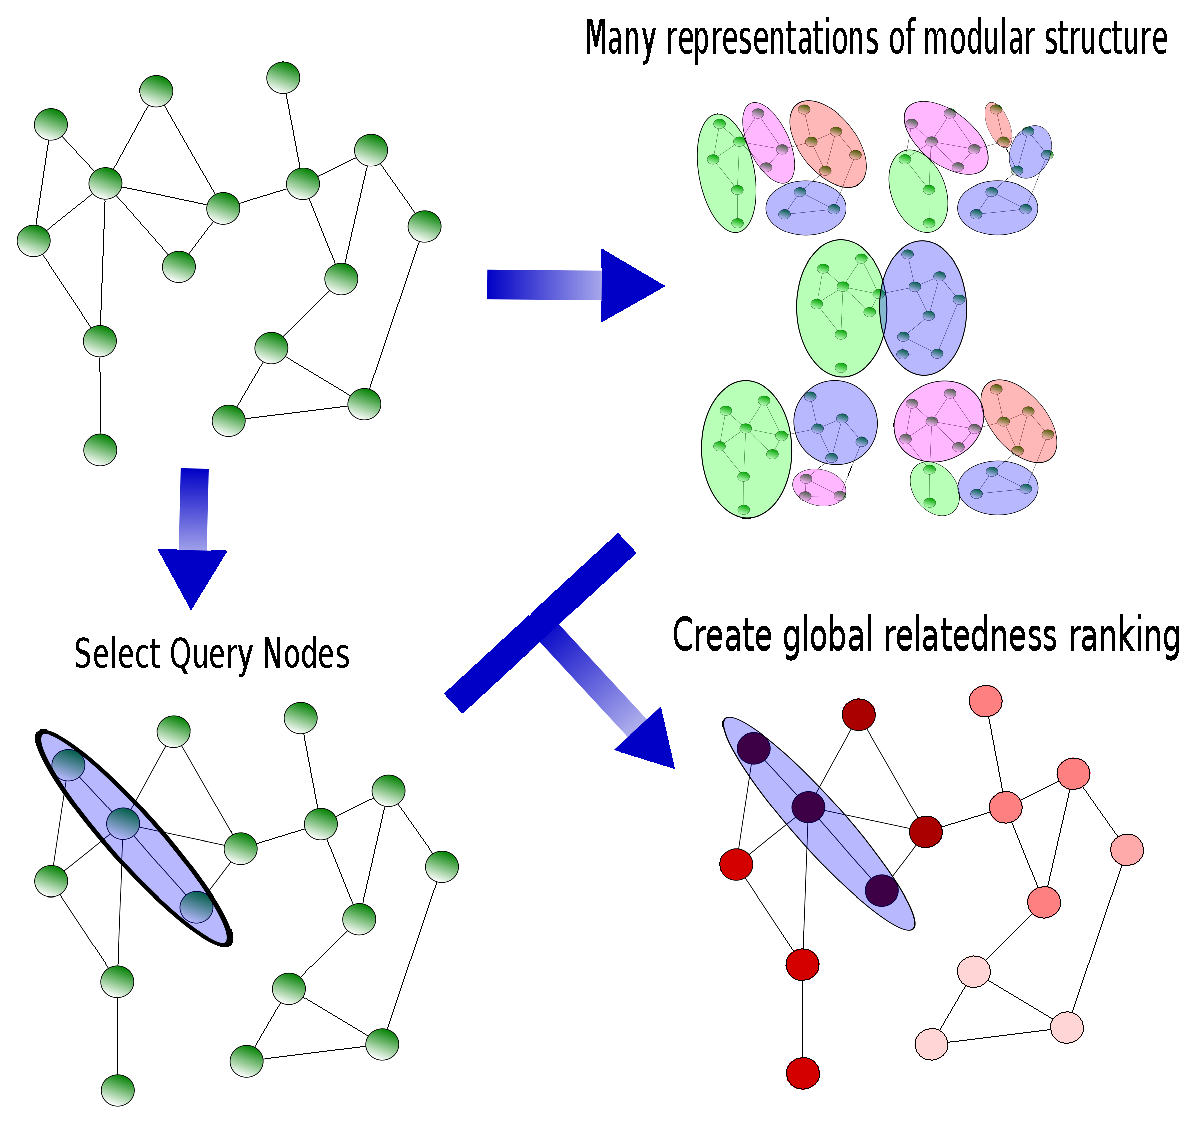
\includegraphics[width=0.6\textwidth]{images/meth_fig/fig1_desc.eps}
 \caption{Outline of the proposed approach to querying networks by using multiple, high quality representations of modular networks.}
 \label{fig:algorithm_outline}
\end{figure*}


\subsection{Generating the search index}
In order to cover the space of high modularity partitions, randomly generated starting partitions are computed with a random cut set.
To achieve this each edge is either placed inside the cut set or not as the result of an independent Bernoulli trial. 
Each random partition is used as the starting partition for the greedy louvain process.
In principle, any search exploration procedure, such as simulated annealing \cite{GuimeraNature2005} could be used.
The Louvain algorithm is selected as it is fast, running in $O(n \log n)$ time complexity \cite{blondel2008fast}, and because it is a greedy algorithm is is guaranteed to stop after finding a locally maximal solution.

The Louvain algorithm is conceptually very simple; starting from a random partition, clusters are agglomerated if the merge results in a positive change in modularity $\Delta Q$.
When no possible moves result in an increase in modularity the algorithm has found a local optima and stops.
Whilst, in principle, the found local optima should have a high modularity score this is not guaranteed.
Consequently, the process here rejects any solutions if the value of modularity is not significantly higher than the distribution of starting partitions.
This is achieved by means of a standard $z$-test, formally the probability of generating a random partition with a modularity score $Q$ as high as observed as a result of the Louvain optimisation must be $p < 0.01$.
Furthermore, only unique solutions are accepted.

The index \textit{coverage} is directly proportional to the number of starting random partitions.
A full coverage index could be considered as every locally optimal partition.
Given that there is no free lunch and it is impossible to know every solution, one can only ensure a full coverage index through an exhaustive search over the $2^m$ possible starting cut sets.
Consequently, in the approach taken here is to use a large but not exhaustive subset of the possible solutions using 10,000 solutions for the large networks studied in this paper.


\subsection{Measuring the quality of relationships} \label{sec:expansion}
Given a query of vertices, the relatedness to other vertexes in a network is quantifiable by the fraction of times they are clustered with the query set, given the set of high quality partitions.
Formally, this can be expressed in terms of the \textit{expansion score} of a given vertex,
\begin{equation} \label{eq:mu_score}
\mu_i(S) = \frac{1}{|\mathcal{P}| |S - i|} \sum_{P \in \mathcal{P}} \sum_{j \in S - i} \delta(c^{P}_{i}, c^{P}_{j}),
\end{equation}
where $S$ denotes a query set, $P$ is a given partition in the space of all high quality partitions $\mathcal{P}$, $c^{P}_{i}$ indicates the partition vertex $i$ is contained in within partition $P$ and $\delta(u, v)$ is the Dirac delta function that equals 1 if vertex $i$ and $j$ are in the same partition and $0$ otherwise.
Borrowing the terminology of fuzzy logic \cite{zimmermann2001fuzzy}, \textit{$\mu_i(S)$} can be considered a membership function and we can interpret this as a measure of the \textit{possibility} for which a given vertex belongs to the query set, given a set of partitions.
Where $\mu_i(S) = 1$ the partition space indicates that a given vertex is always partitioned in the same group as the query set.
In the case $\mu_i(S) = 0$ the vertex $i$ never appears in the same cluster as any vertex in the query set.

The subtraction of the vertex from the query set ($S - i$) allows an unbiased score for vertices within the query set.
This allows us to define a vector, $\mu(S)$ for all vertices in the network, including those in $S$.

\section{Results}
\subsection{Cross-validation method}
\label{sec:cross_validation}
In this work we are presented with a problem of a small number of labels for true positive cluster information.
The cross validation procedure we devise is described as follows and depends on the size of the community and the number of initial seed labels being used.
For this work we would like to capture binary classification  performance, \textit{true positives (tp), true negatives (tn), false positives (fp)} and \textit{false negatives (fn)}, on our datasets.
As the seed label sets can be as small as 3 vertices, exhaustive cross validation is not possible for all labelling schemes.
Consequently, cross validation is either conducted on an exhaustive set of all possible $\binom{|L|}{s}$ unique labellings or 120 seed queries sampled without replacement, where $L$ is the set of gold standard true labels and $s$ is the size of the randomly selected seed sets.
It should therefore be noted that presented receiver operator characteristic (ROC) scores are, therefore, dependent on community sizes.

\subsection{Synthetic networks}
In this section we test the method on a number benchmark networks constructed with a known, ground-truth community structure.
To evaluate how our method performs we demonstrate results against two benchmark networks the conventionally used LFR benchmark \cite{lfr} and a newer form of benchmark for community detection algorithms developed in previous studies \cite{cigram}.
Both these benchmarks allow for a configurable level of overlapping and mixing between communities.

\subsubsection{LFR benchmarks}

\subsubsection{CiGRAM benchmarks}

\subsection{Real networks}
In order to test the performance of the semi-supervised classification on real-world data we present our findings on example networks with known metadata communities.
All datasets taken use the largest single connected component sub-graph.

\subsubsection{Dataset descriptions}
\label{sec:real_network_descs}
The real networks used are listed as follows:
\begin{itemize}
 \item \textbf{EU emails dataset (EU emails)} This anonymised dataset is taken from the SNAP database \cite{snap} and contains $986$ nodes and $16,687$ edges representing emails between individuals.
 The metadata community labels represent different departments within the organisation.
 In total there are 42 communities, 39 of which contain at least 3 nodes.
 
 \item \textbf{Yeast protein-protein interaction network (Yeast PPI)} \cite{yeast_ppi}
 This dataset is a collection of recorded binary interactions between proteins collected with high-throughput yeast-2-hybrid assays.
 The metadata used are known, experimentally validated protein complexes from \cite{yeast_ppi_complexes}.
 The network contains 6222 nodes in the largest connected component, with 22,3868 edges.
 There are 409 experimentally validated protein complexes, 236 of which contain 3 or more nodes.
 The protein complexes are typically very small in terms of number of proteins with only 90\% of the complexes containing less than 10 proteins and only 2 complexes containing 50 or more proteins.
 
\end{itemize}

\begin{figure}[ht]
     \centering
    \begin{subfigure}[b]{\textwidth}
        \centering
        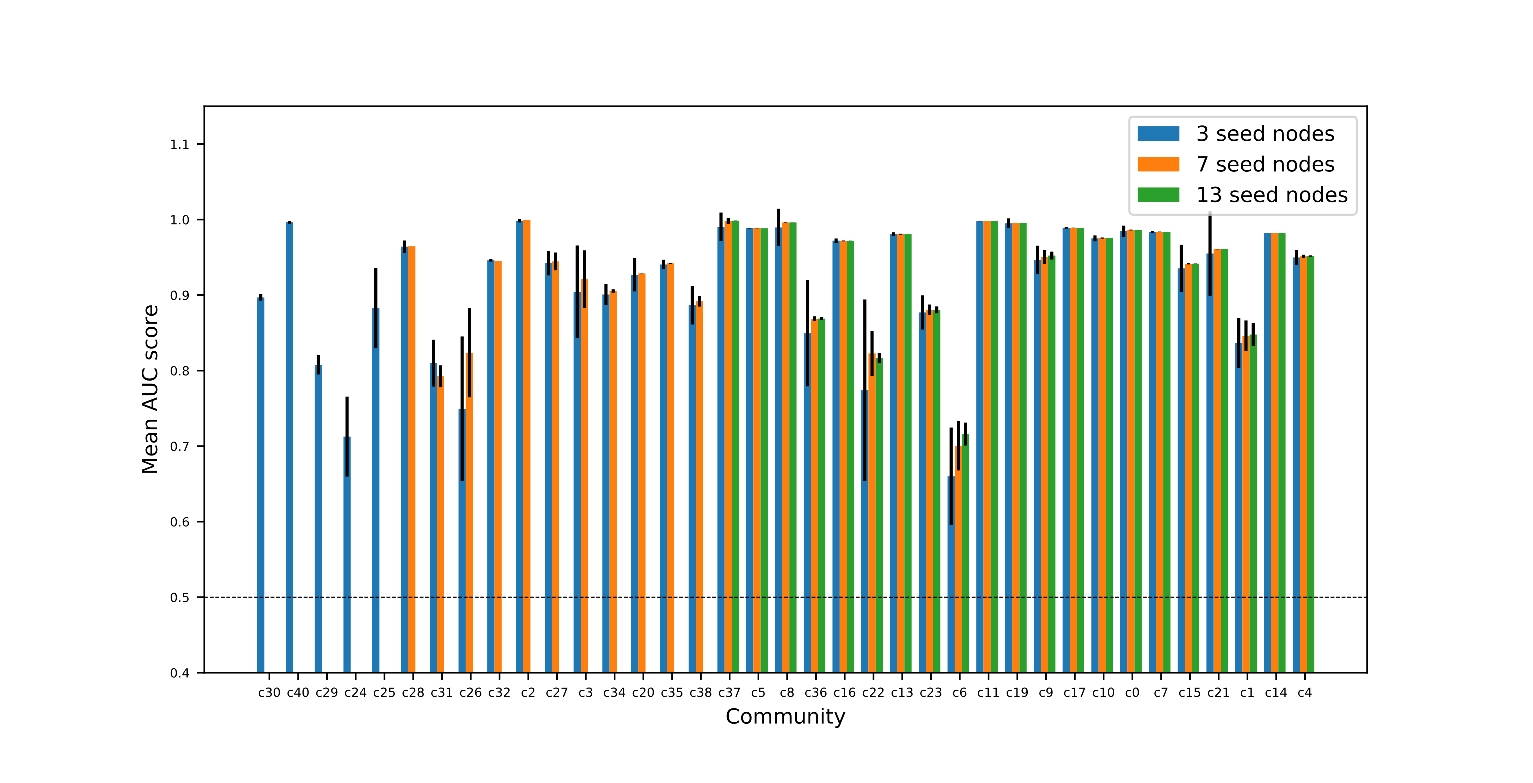
\includegraphics[width=\textwidth]{images/eu_roc_scores.eps}
        \caption{EU email departments}
    \end{subfigure}
    
    \centering
    \begin{subfigure}[b]{\textwidth}
        \centering
        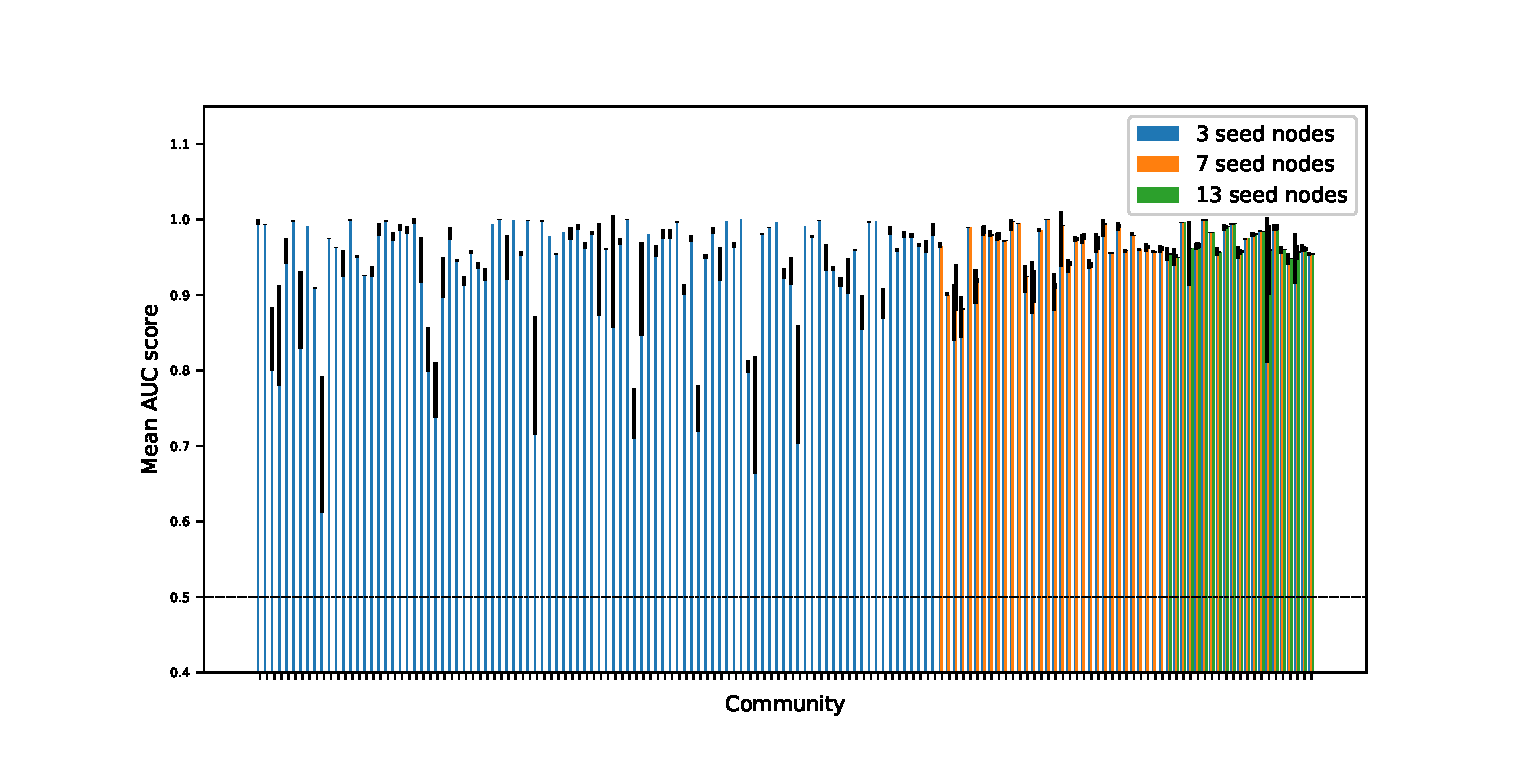
\includegraphics[width=\textwidth]{images/yeast_ppi_roc_scores.eps}
        \caption{Yeast PPI protein complexes}
    \end{subfigure}
    
    \caption{Mean area under RO curve (AUC) scores from cross-validation performed on Metadata communities for networks described in Section \ref{sec:real_network_descs}.
    Dashed line indicates an AUC score of 0.5 (random chance).
    Communities are ordered by size.
    Error bars indicate standard deviation.
    }
    \label{fig:real_network_results}
\end{figure}

\begin{figure}[ht]
     \centering
    \begin{subfigure}[b]{0.8\textwidth}
        \centering
        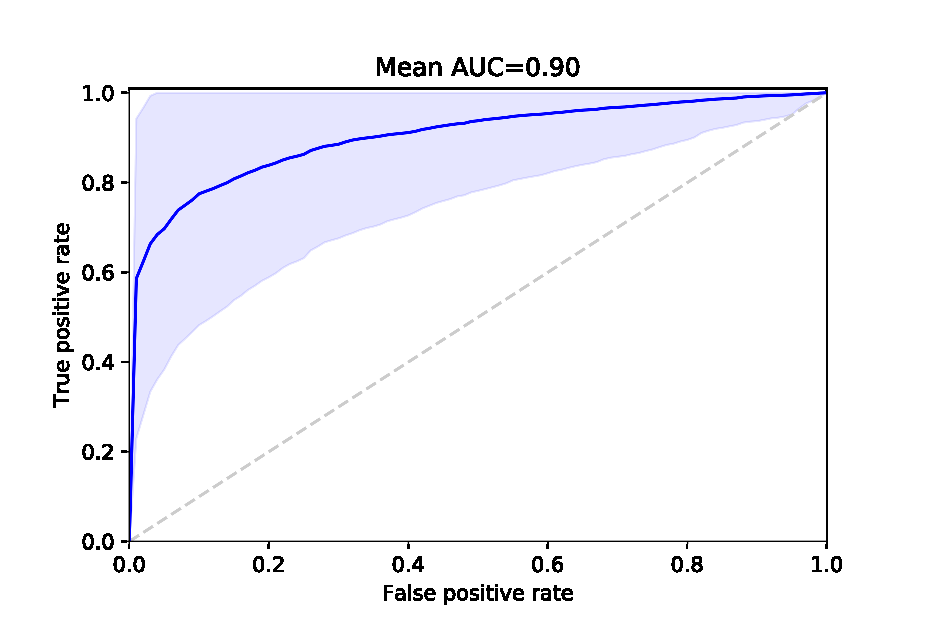
\includegraphics[width=\textwidth]{images/eu_email_nodewise_roc.eps}
        \caption{EU email departments (986 nodes)}
    \end{subfigure}
    
    \centering
    \begin{subfigure}[b]{0.8\textwidth}
        \centering
        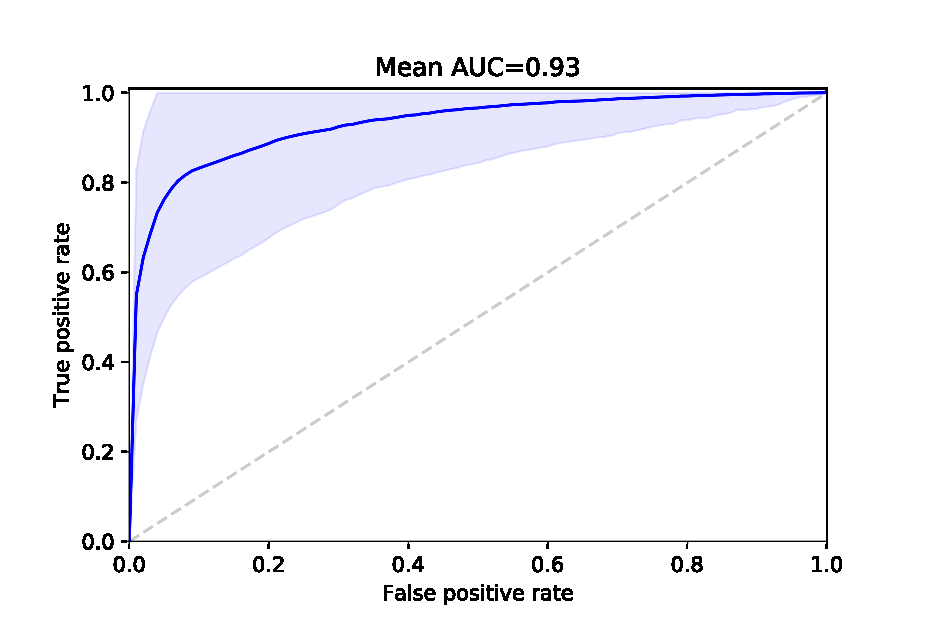
\includegraphics[width=\textwidth]{images/yeast_ppi_nodewise_roc.eps}
        \caption{Yeast PPI protein complexes (1628 nodes)}
    \end{subfigure}
    
    \caption{Receiver Operator Characteristic curves for node communities.
    Dashed line indicates an AUC score of 0.5 (random chance).
    Represents mean, shaded area indicates standard deviation.
    }
    \label{fig:real_network_nodwise_classifiers}
\end{figure}


We tested the method on each real network described in section \ref{sec:real_network_descs}.
Figure \ref{fig:real_network_results} shows the mean ROC scores for each community in the relevant networks, organised by size of community at increasing numbers levels of query seed nodes.
On the EU emails and Yeast PPI dataasets, for all communities tested with 3 or more nodes, mean AUC scores calculated with the cross validation method described in section \ref{sec:cross_validation} were above 0.6.
There appeared to be no statistically significant improvements to using more than 3 seed nodes.

The classification for individual nodes is presented in Figure \ref{fig:real_network_nodwise_classifiers}.
Here, binary classification is performed on each node for which community data is available.
The $mu_i({i})$ score is used as a binary classifier.
For the EU email and Yeast PPI the average ROC AUC score to classify node membership inside communities is 0.9 and 0.93, respectively.

\section{Discussion}
The semi-supervised method for vertex classification presented in this work has shown to have good results on both synthetic benchmarks and real-world datasets.
Interestingly, this method is capable of correctly classifying communities with only a small number of seed query vertexes.
These results show that the community query method could be used as a powerful exploratory tool in network analysis.

The fact that the method is able to uncover small protein complexes seems to contradict the principle that modularity maximisation algorithms have a resolution limit \cite{}.
This may be due to the fact that
We do note that, where communities are very small, any approach will extremely sensitive to false positive and false negative results.
This should be considered when using this method as an exploratory tool.

The results also appear to be highly tolerant to a small number of seed nodes.
This is interesting as in most sampled cases the relevant nodes are unlikely to be direct neighbours.
From the perspective of exploratory study, this implies that a small number of query vertices can be used to find potentially related vertices.

This allows the use of a single node to find related vertices, in real networks the results appeared to have a very good level of accuracy with average AUC of ROC curves above $0.9$.
In a practical context, however, this should not be interpreted as uncovering the community structure as this includes many overlapping communities for which the node is a member.



\section{Related work}
\label{sec:related_work}

This work relates very strongly to the idea of local community detection, more specifically the idea of \textit{seed set expansion}.
Here, a given seed set is created a random walks are analysed to find clearly related communities of vertices.
One of the most common approaches to finding related vertices in a network is the random walk with restart (RWR) \cite{can2005analysis, kohler2008walking}.
This approach has been applied in fields as diverse as recommender systems and the detection of potential drug targets \cite{chen2012drug}.
In RWR the relatedness of any pair of vertices can be seen as the probability of a particle traversing the graph starting at a given vertex and ending at another.
The restart aspect of the random walk can be thought of as the probability of the walker teleporting back to the start vertex with some none zero probability. 
The higher the probability of the walker ending up at a given vertex, the more likely it is that the two vertices are related.

Conceptually, RWR is very similar to the method presented in this paper given that the user has a given query.
One can thing of the RWR probability as analogous to the value of $\mu_i(S)$ presented above.
However, the RWR value is based only on a single vertex as a query set where the approach presented in this work requires many vertices associated with a given label for it to be readily applicable.


Many existing method are based on the idea of a locally dense subgraph containing \textit{all query nodes} \cite{}.
In contrast, the query approach presented here does not require the queries to be a self contained sub-graph.
Indeed, queries can contain spurious nodes that are topologically distinct from one another - the result is that the either $q(S)$ score for the query will be very low and insignificant, or the spurious nodes will be ignored in the final query set.
In user facing domains it is highly likely that very large query sets do not form isolated topologies.
With Conventional methods some ``cleaning up'' of the underlying queries is often required to gather any meaningful expansion.

Whilst modularity maximisation is used for the set of global partitions, this approach is distinct from local modularity based approaches \cite{}.
A limitation of this approach compared with localised methods is that the entire dataset is required.
However, the objective is somewhat different as the approach presented here relies on high quality meta-data labels for queries.
In this sense, the approach should be considered closer to semi-supervised \textit{classification} than unsupervised \textit{clustering}.

In the field of community detection, a number of very recent articles have focused on using metadata to improve the results of community detection approaches.

%TODO: Discuss citations of metadata based community detection - Newman-Clauset, Jure Lesovec, other citations in newman paper.

These algorithms, however, are distinct from the approach taken here as the metadata is not used in the module discovery process.
Furthermore, the results in this work attempt to explicitly label unlabelled data and only require a relatively small number of labels to operate in such a fashion.
In contrast,  the recent approach by Newman and Clauset \cite{}, for example, uses examples in which practically the entire network contains labels which is less useful from the perspective of label discovery.
However, these methods are vastly superior to the work presented here when considering the research question of whether a labelling scheme (such as demography in a social network) accurately describes the structure of the network. 

\section{Conclusions}
This paper has presented a novel approach to semi-supervised community detection utilising a consensus of high scoring partitions computed with the popular modularity maximisation approach.
Previously the glassy search space of this optimisation algorithm has been seen as a major limitation of the approach.
However, in this work we consider each locally optimal partition to be information regarding the true multi-class labels that are likely present in real networks.
As the algorithm is trivial to run in a distributed manner, this approach can be applied to relatively large graphs.
Further research can be conducted into this approach with alternative quality functions to modularity that do not suffer the same limitations in terms of a resolution limit.

However, this approach requires the community landscape to contain many local maxima, a property likely shared by many real networks.
Similarly, the method presented here requires both some labelled data and the labels to be represented well within the topology of the underlying network.
The approach presented here differs from other ensemble approaches in that the objective is to provide a probabilistic framework for label classification.
This approach performs extremely well on both synthetically generated networks and real-world ground truth communities with relatively small sets of labels.

% Furthermore, we extended the use of this framework to allow quality measurements of selected labellings and similarity comparrisons between data.

\section*{Acknowledgements}
We are grateful for access to the University of Nottingham High Performance Computing Facility for supporting this work.
This work was supported by the Biotechnology and Biological Sciences Research Council grant BB/L013940/1.

\bibliographystyle{IEEEtran} 
\bibliography{references}

% \nocite{*}
\end{document}
